\chapter{Vybrané zbernicové protokoly}
\label{kap:zbernice}

V tejto kapitole stručne spomenieme vybrané zbernicové protokoly a zhrnieme ich kľúčové vlastnosti, ktoré budú relevantné v ďalších častiach práce. Vo všeobecnosti existuje mnoho rôznych zbernicových protokolov. Tie môžu využívať rôzne techniky, ktoré umožňujú zabezpečiť komunikáciu a jej riadenie. Mnoho týchto protokolov má však veľa spoločných znakov. Aj preto sa v práci budeme venovať iba niektorým vybraným. V tejto kapitole najskôr uvedieme niektoré základné vlastnosti zberníc. Následne predstavíme 3 príklady zberníc (UART, SPI, I\textsuperscript{2}C), ktorých podporu implementujeme na FPGA MITM obvode popísaného v kapitole \ref{kap:implementacia}.

\section{Vlastnosti hardvérových zberníc}
V tejto časti spomenieme vybrané vlastnosti hardvérových zberníc a základnú kategorizáciu na základe týchto vlastností. Vlastnosti, ktoré opíšeme sú relevantné pre spôsob implementácie hardvérového MITM útoku na danej zbernici.

\subsection{Synchrónne a asynchrónne zbernice}
Pre účel MITM útoku je veľmi dôležité rozlišovať medzi tzv. synchrónnymi a asynchrónnymi zbernicami. Synchrónne zbernice sa vyznačujú tým, že dátový signál je doplnený o synchrónny hodinový signál, ktorý riadi prenos dát na zbernici a umožňuje správne prečítať a dekódovať prenášané dáta. Takýto signál môže byť explicitne vysielaný na samostatnej linke, napr. zbernice SPI a I\textsuperscript{2}C.

Iný spôsob ako preniesť hodinový signál je zakódovať hodinový signál vrámci dátového. Prijímajúce zariadenie dokáže následne z prijatého signálu správne dekódovať synchrónne dáta. Tento spôsob prenosu synchrónnych dát sa využíva najmä pri vysokorýchlostných (angl. high-speed) sériových zberníc \cite{serdes}, tzv. SerDes (Serializer-Deserializer), ako sú napríklad USB a PCIe \cite{pcieSpec}. Vysokorýchlostným zberniciam sa v práci nebudeme venovať, nakoľko si na fyzickej vrstve vyžadujú dedikovaný hardvér a vrámci FPGA obvodov sa zvyknú implementovať iba vyššie vrstvy daných protokolov.

Protikladom synchrónnych zberníc sú asynchrónne zbernice.

\subsection{Architektúra master-slave}

\subsection{Ďalšie vlastnosti zberníc}
Simplex, half-duplex, full-duplex\\
point-to-point vs broadcast\\
Sériové a paralelné zbernice

\section{UART zbernica}
UART (Universal Asynchronous Receiver Transmitter) je defakto-štandard, ktorý okrem hardvérového rozhrania čiastočne definuje aj komunikačný protokol a niektoré jeho parametre. Z hľadiska kategorizácie ide o asynchrónnu linku

\section{SPI Zbernica}
Zbernica SPI je defakto-štandard, ktorý definuje hardvérové rozhranie, pre zapojenie komunikujucích strán. Podobne ako I$^2$C, ide o bitovo orientovanú synchrónnu linku. Keďže ide o defakto-štandard, zbernica SPI nedefinuje predpísanú štruktúru posielaných dát \cite{spiBus}.

\subsection{Riadenie prístupu k zbernici}
Podobne ako pri I$^2$C zbernici, komunikácia je riadená master-slave architektúrou. Prístup k zbernici riadi master prostredníctvom dedikovaného vodiča SS (Slave Select) pre každé slave zariadenie. Vodiče SS zvyknú byť označené aj ako CS (Chip Select). V pasívnom stave je na každom SS vodiči logická hodnota 1. Pred začatím komunikácie s vybraným slave zariadením nastaví master logickú hodnotu 0 na príslušnom SS vodiči, čím umožní komunikáciu medzi master a príslušným slave zariadením. Tento spôsob riadenia zbernice vytvára ilúziu point-to-point linky medzi komunikujúcimi stranami, preto v zbernici SPI nie je potrebná adresácia.

\subsection{Hardvér SPI zbernice}
SPI zbernica pozostáva z troch hlavných liniek: MISO (Master In Slave Out), ktorý zabezpečuje prenos dát smerom od slave zariadení k master zariadeniu, MOSI (Master Out Slave In) pre prenos dát opačným smerom a SCLK (Serial Clock) pre prenos hodinového signálu (generovaný master zariadením) \cite{spiBus}. Schéma zapojenia pomocou SPI zbernice je na obrázku \ref{obr:spiWiring}. Dáta po vodičoch MISO a MOSI môžu tiecť súčasne čo umožňuje full-duplex komunikáciu.

\begin{figure}
    \centerline{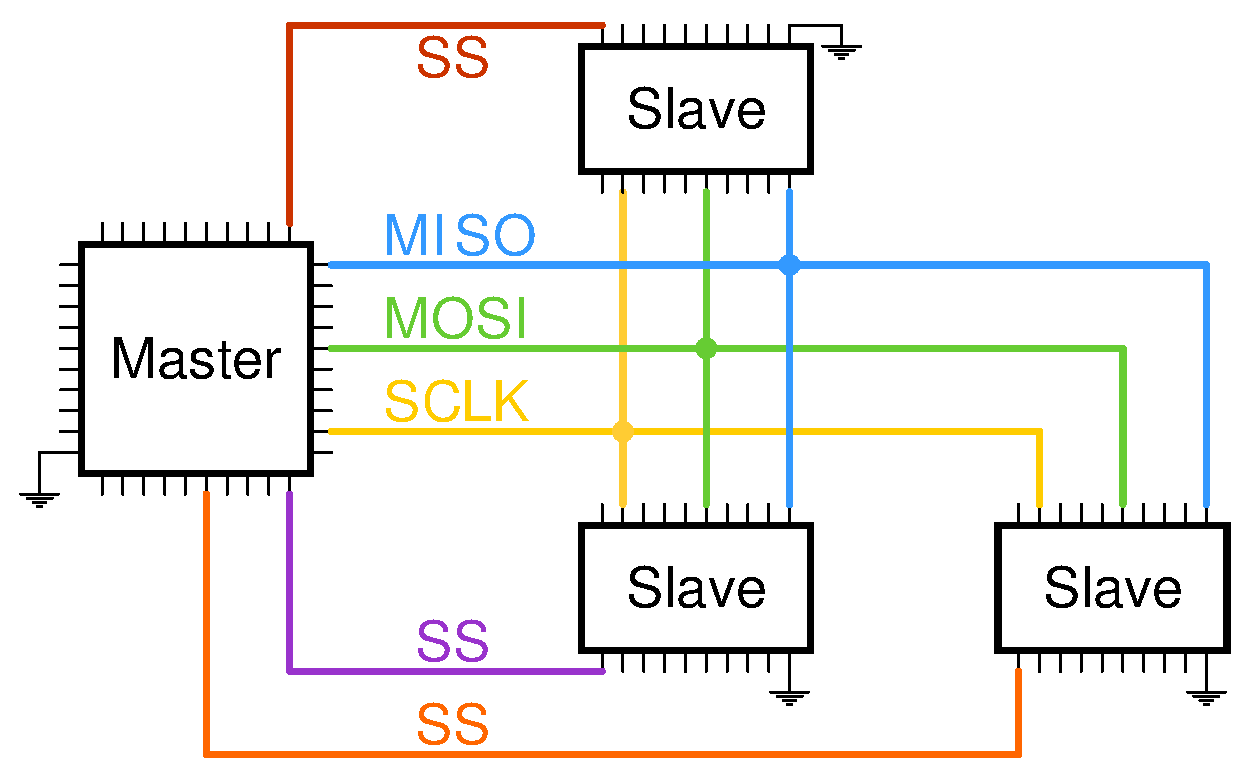
\includegraphics[width=0.9\textwidth]{images/spiWiring.png}}
    \caption[Zapojenie zbernice SPI]{Zapojenie zbernice SPI.}
    \label{obr:spiWiring}
\end{figure}

\section{I\textsuperscript{2}C zbernica}
I$^2$C (Inter-Integrated Circuits) je štandardizovaná zbernica, vyvinutá spoločnosťou Philips Semiconductors, určená pre jednoduchú komunikáciu medzi integrovanými obvodmi \cite{i2cSpec} väčšinou v rámci jednej dosky plošných spojov. Ide o bitovo-orientovanú synchrónnu linku, čo znamená, že komunikácia je synchronizovaná hodinovými impulzmi a prenášaná dátová jednotka je bit.

\subsection{Hardvér I\textsuperscript{2}C zbernice}
Zbernica pozostáva z dvoch vodičov: SDA (Serial Data Line), ktorý zabezpečuje sériový prenos dát (bitov) a SCL (Serial Clock Line) pre prenos synchronizačného hodinového signálu \cite{i2cSpec}. Vodiče sú na komunikujúcich zariadeniach pripojené v tzv. open-drain režime a (každé zvlášť) sú cez zdvíhací odpor (pull-up rezistor) pripojené k napätiu 5\,V resp. 3.3\,V v závislosti od konfigurácie. Na obrázku \ref{obr:i2cWiring} je znázornené zapojenie zariadení pomocou zbernice I$^2$C.

\begin{figure}
    \centerline{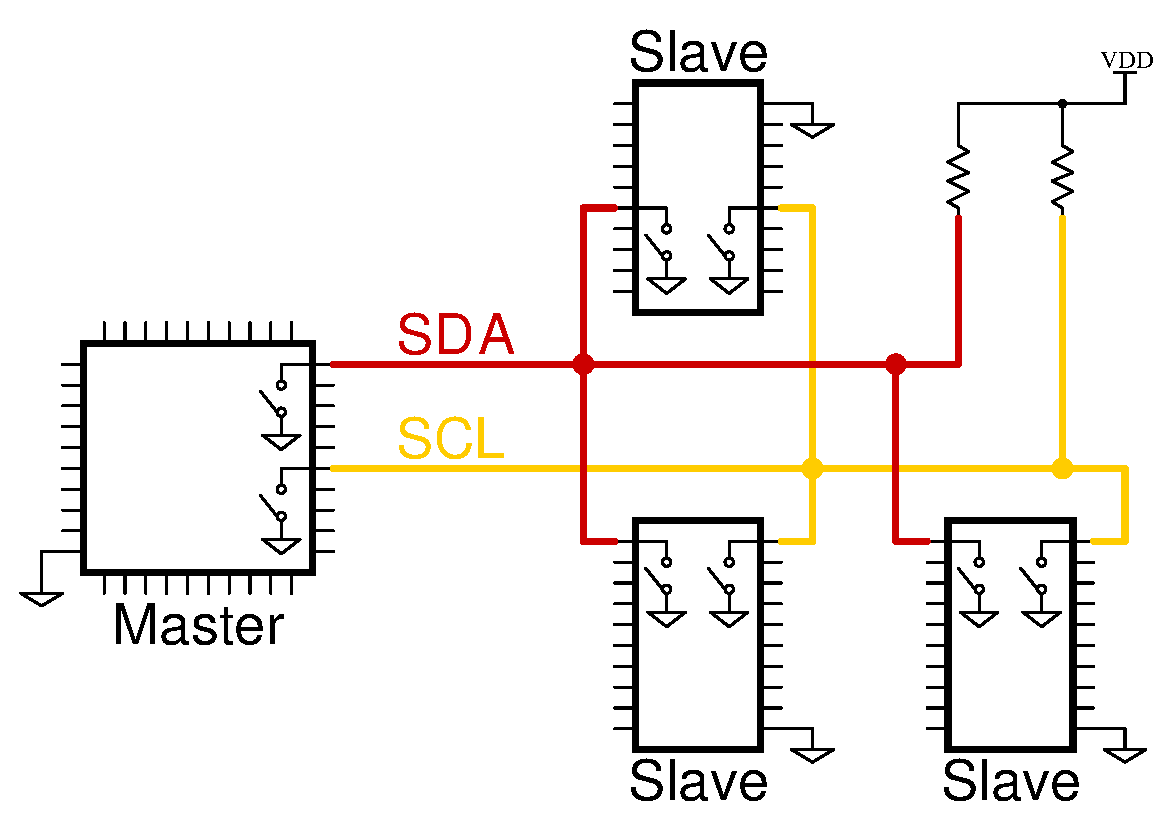
\includegraphics[width=0.9\textwidth]{images/i2cWiring.png}}
    \caption[Zapojenie zbernice I$^2$C]{Zapojenie zbernice I$^2$C. Open-drain logika interného zapojenia vodičov v zariadeniach je znázornená pomocou \uv{spínačov}. V skutočnosti je realizovaná pomocou tranzistorov.}
    \label{obr:i2cWiring}
\end{figure}

V pasívnom stave je teda na vodičoch hodnota napätia 5\,V (resp. 3.3\,V), čo na dátovej linke zodpovedá logickej hodnote 1. V prípade, že práve vysielajúce zaradenie chce poslať bit s logickou hodnotou 0, \uv{pripojí} (napr. pomocou tranzistora) vodič na spoločnú zem, čím napätie klesne na 0\,V. Dáta na vodiči SDA sú vzorkované pri nábehovej hrane na SCL signálovej linke \cite{i2cSpec}.

\subsection{Riadenie prístupu k zbernici}
Zbernica I$^2$C je typu half-duplex, podporuje teda obojsmernú komunikáciu, pričom súčasne môže komunikácia prebiehať iba jedným smerom. Komunikácia na I$^2$C zbernici je riadená architektúrou master-slave \cite{i2cSpec}. Master zariadenie riadi komunikáciu na hardvérovej aj protokolovej úrovni. Na hardvérovej úrovni master zariadenie určuje rýchlosť komunikácie generovaním hodinových impulzov na SDL vodiči. Zbernica podporuje rôzne konfigurácie, ktoré sa líšia rýchlosťou rádovo od 100\,kbps až po niekoľko\,Mbps. Na protokolovej úrovni je každá komunikácia iniciovaná aj ukončená master zariadením a slave zariadenia musia synchrónne posielať dáta vo vyhradených časoch, ktoré definuje protokol.

\subsection{Protokol a štruktúra rámcov}
I$^2$C je zbernica so zdieľaným médiom, čo znamená, že umožňuje na spoločnú zbernicu pripojiť viacej než dva komunikujúce uzly. Je preto potrebné zabezpečiť adresáciu jednotlivých zariadení, s ktorými chce master nadviazať komunikáciu. Každé slave zariadenie má pridelenú 7-bitovú (resp. 10-bitovú v novšej verzii štandardu) adresu, ktorá je zvyčajne zadrôtovaná výrobcom hardvéru \cite{i2cSpec}. Z dôvodu predchádzania kolízií v adresách, zvyknú výrobcovia prideliť zariadeniu viacero adries, z ktorých je možne nakonfigurovať práve jednu, väčšinou hardvérovým spínačom.

Samotná komunikácia vyzerá nasledovne: Master zariadenie nastaví úroveň napätia na SDA linke na hodnotu logickej 0, čím pošle tzv. START bit, ktorý signalizuje začiatok komunikácie. Nasleduje 7-bitová (resp. 10-bitová) adresa zariadenia, s ktorým chce master komunikovať a jeden tzv R/W bit, ktorý označuje, či ide o operáciu čítania alebo zápisu. (Z pohľadu master zariadenia logická 1 predstavuje čítanie, 0 predstavuje zápis.) S nasledujúcim hodinovým impulzom musí adresované slave zariadenie komunikáciu potvrdiť (pošle tzv. ACK bit) tým, že úroveň napätia na SDA linke nastaví na hodnotu logickej 0. Potom nasledujú samotné dáta, ktoré posiela master (resp. slave v prípade, že ide o operáciu čítania). Dáta su členené na 8-bitové sekvencie, ktoré sú zakaždým potvrdzované druhou stranou rovnakým spôsobom. Za posledným potvrdením dát pošle master tvz. STOP bit, čím signalizuje ukončenie komunikácie. Štruktúra rámca je znázornená na obrázku \ref{obr:i2cFrame}.

\begin{figure}
    \centerline{\includegraphics[width=1\textwidth]{images/i2cFrame.png}}
    \caption[Štruktúra I$^2$C rámca]{Štruktúra I$^2$C rámca.}
    \label{obr:i2cFrame}
\end{figure}

V prípade, že počas komunikácie nastane chyba, prijímajúce zariadenie nepošle ACK bit. Teda napätie na SDA linke ostane na úrovni logickej 1 (tzv. NACK bit), čo je zároveň pasívny stav. V takomto prípade môže master reagovať dvoma spôsobmi. Buď pošle STOP bit, čo znamená okamžité ukončenie komunikácie, alebo môže zopakovať komunikáciu od začiatku, tým, že pošle START bit. Postupnosť NACK a STOP môže byť master zariadením zároveň využitá na signalizáciu ukončenia komunikácie v prípade operácie čítania \cite{i2cSpec}.

\subsection{Mechanizmus naťahovania hodín}
Naťahovanie hodín (angl. clock stretching) je mechanizmus I$^2$C protokolu, ktorý umožňuje slave zariadeniu dočasne spomaliť hodinové impulzy generované master zariadením \cite{i2cSpec}. To umožňuje slave zariadeniu spomaliť rýchlosť komunikácie, v prípade potreby väčšieho času pre spracovanie dát.

Počas prebiehajúcej komunikácie master zariadenie monitoruje vysielaný hodinový signál na SCL linke. Pripomíname, že vodič SCL linky je pripojený cez zdvíhací odpor k zdroju napätia a komunikujúce zariadenia majú vodič pripojený v open-drain režime. Pokiaľ chce slave zariadenie spomaliť komunikáciu môže podržať SCL vodič pripojený na zem, čím dosiahne efekt, že napätie na vodiči ostane na úrovni logickej 0 aj v prípade, že master posiela logickú 1. Tento stav dokáže master detegovať a následne prispôsobiť rýchlosť hodinových impulzov, čím spomalí komunikáciu. Mechanizmus naťahovania hodín je znázornený na obrázku \ref{obr:i2cStretch}.

\begin{figure}
    \centerline{\includegraphics[width=0.8\textwidth]{images/i2cStretch.png}}
    \caption[Mechanizmus naťahovania hodín]{Mechanizmus naťahovania hodín. Na vrchnej časti je pôvodný hodinový signál vysielaný master zariadením. Na spodnej je skutočný signál po natiahnutí hodín slave zariadením.}
    \label{obr:i2cStretch}
\end{figure}